\documentclass[tikz,border=6pt]{standalone}
\usepackage[T1]{fontenc}
\usepackage{lmodern}
\usetikzlibrary{arrows.meta,positioning,shapes.geometric,fit,calc,backgrounds}
\definecolor{ink}{HTML}{292642}
\definecolor{violet}{HTML}{7054DC}
\definecolor{violetlight}{HTML}{F1EDFF}
\definecolor{teal}{HTML}{147D77}
\definecolor{teallight}{HTML}{E8F5F3}
\definecolor{amber}{HTML}{9A641F}
\definecolor{amberlight}{HTML}{FFF3DE}
\definecolor{linegray}{HTML}{A7A9BA}
\tikzset{box/.style={draw=violet!55,fill=violetlight,rounded corners=3pt,minimum width=2.25cm,minimum height=0.8cm,align=center,font=\sffamily\scriptsize,text=ink,inner sep=5pt},actual/.style={box,draw=teal!70,fill=teallight},proposed/.style={box,dashed,draw=amber!75,fill=amberlight},small/.style={font=\sffamily\tiny,text=ink,align=center},lab/.style={font=\sffamily\scriptsize\bfseries,text=ink},flow/.style={-{Stealth[length=2mm]},line width=.8pt,draw=violet},dflow/.style={flow,dashed,draw=amber},boundary/.style={draw=linegray,dashed,rounded corners=4pt,inner sep=8pt}}
\begin{document}

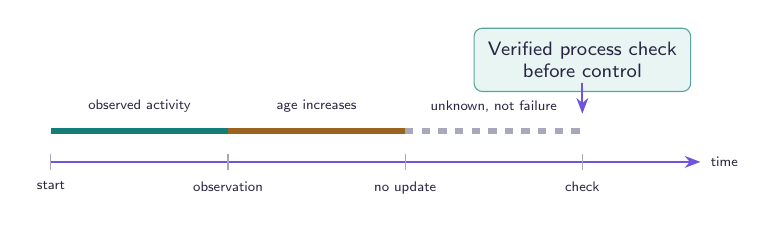
\begin{tikzpicture}[x=.75cm,y=.72cm]
\draw[flow] (0,0)--(11,0) node[right,small]{time};
\foreach \x/\lab in {0/start,3/observation,6/no update,9/check} {\draw[draw=linegray] (\x,.14)--(\x,-.14);\node[small,below] at (\x,-.18) {\lab};}
\draw[line width=2.2pt,draw=teal] (0,.55)--(3,.55);
\draw[line width=2.2pt,draw=amber] (3,.55)--(6,.55);
\draw[line width=2.2pt,draw=linegray,dashed] (6,.55)--(9,.55);
\node[small,above] at (1.5,.7) {observed activity};
\node[small,above] at (4.5,.7) {age increases};
\node[small,above] at (7.5,.7) {unknown, not failure};
\node[actual] at (9,1.8) {Verified process check\\before control};
\draw[flow] (9,1.4)--(9,.85);
\end{tikzpicture}
\end{document}
